% Include all the tex files needed to compile the document
\documentclass[a4paper,twoside,11.5pt]{scrbook}

% Include
% List of packages to include
\usepackage[english]{babel}
\usepackage{graphicx}
\usepackage[dvipsnames]{xcolor}% http://ctan.org/pkg/xcolor
\usepackage{amssymb}
\usepackage{amsbsy}
\usepackage{amsmath}
\usepackage[colorlinks=true,bookmarks=false,linkcolor=blue,urlcolor=RoyalBlue,citecolor=magenta, backref=page]{hyperref}
\usepackage[acronyms]{glossaries}
\usepackage[nameinlink,capitalise,noabbrev]{cleveref}
\usepackage[singlespacing=true]{scrlayer-scrpage}

% Style of the document

% Margins
\usepackage{vmargin}
\setpapersize{A4}
\setmarginsrb{3cm}{3cm}{3cm}{2cm}{6mm}{7mm}{5mm}{15mm}
\setlength{\marginparwidth}{2cm}

% Sections
\setkomafont{chapter}{\Huge\rmfamily\color{RoyalBlue}}
\setkomafont{section}{\LARGE\rmfamily\color{RoyalBlue}}
\setkomafont{subsection}{\Large\rmfamily\color{RoyalBlue}}
\setkomafont{subsubsection}{\large\rmfamily\color{RoyalBlue}}
\renewcommand*{\chapterformat}{{\color{RoyalBlue}\thechapter}}
\renewcommand\chapterlinesformat[3]{#2\par#3\vspace{5cm}}

% Paragraphs
\parindent 0cm % Do not indent beginning of paragraph
\parskip1.5ex plus0.5ex minus0.5ex % Margin between paragraphs
\renewcommand{\baselinestretch}{1.25} 

% Headers
\usepackage{scrlayer-scrpage}
\pagestyle{scrheadings}
\lehead{{\headfont\thepage}} % Left/right header for even/odd pages
\rohead{{\headfont\thepage}} % Left/right header for even/odd pages
\lohead{\headfont\uppercase{\rightmark}} % Header for left page (odd)
\rehead{\headfont\uppercase{\leftmark}} % Header for right page (even)
\cfoot{}
\lefoot{}
\rofoot{}

% Captions, footnotes
\usepackage{caption}
\captionsetup{labelfont={color=RoyalBlue,bf},justification=RaggedRight, format=plain, font=small}
\deffootnote[2em]{0em}{1em}{\thefootnotemark.\ }

% Back reference
% See tex.stackexchange.com/questions/15971
\renewcommand*{\backref}[1]{}
\renewcommand*{\backrefalt}[4]{%
    \ifcase #1 %
    \or        (cited on page~#2)%
    \else      (cited on pages~#2)%
    \fi}

% Refer to subsection and subsubsection as "section"
\addto\extrasenglish{
\renewcommand{\chapterautorefname}{Chapter}
\renewcommand{\sectionautorefname}{Section}
\let\subsectionautorefname\sectionautorefname
\let\subsubsectionautorefname\sectionautorefname}

% Abstract
\newenvironment{abstractpage}[1]
{
\clearpage
\thispagestyle{empty}
{\vspace*{1.0cm}\Huge\color{RoyalBlue}\textbf{#1}}
\par\bigskip
}{\clearpage}

% Define shortcut commands

% Mathematical environments
\def \be {\begin{equation}}
\def \ee {\end{equation}}
\def \ba {\begin{equation} \begin{aligned}}
\def \ea {\end{aligned} \end{equation}}
\def \begm {\left(\begin{matrix}}
\def \endm {\end{matrix}\right)}
% \def\sectionautorefname{Section}

% Mathematical symbols
\def \real {\mathbb{R}}

% Fraction with text
\newcommand*\textfrac[2]{
  \ensuremath{\frac{\text{#1}}{\text{#2}}}
}

% Helpers for tables
\newcommand{\Tstrut}{\rule{0pt}{2.6ex}}         % = `top' strut
\newcommand{\Bstrut}{\rule[-0.9ex]{0pt}{0pt}}   % = `bottom' strut
\newcommand{\toprule}{\hline\Bstrut}
\newcommand{\midrule}{\hline\Tstrut\Bstrut}
\newcommand{\bottomrule}{\hline\Tstrut}

% Deal with missing figures which are not directly included in the repository
% Taken from https://tex.stackexchange.com/questions/39982/use-default-figure-if-file-is-missing
\newcommand{\noimage}{%
  \setlength{\fboxsep}{-\fboxrule}%
  \fbox{\phantom{\rule{10pt}{10pt}}Figure missing\phantom{\rule{10pt}{10pt}}}% Framed box
}
\let\includegraphicsoriginal\includegraphics
\renewcommand{\includegraphics}[2][width=\textwidth]{\IfFileExists{#2}{\includegraphicsoriginal[#1]{#2}}{\noimage}}


% Acronyms
% \makeglossaries
\makenoidxglossaries
\newglossaryentry{ML}{
    name={ML},
    description={Machine Learning},
    plural={MLs}
}

\newglossaryentry{DL}{
    name={DL},
    description={Deep Learning},
    plural={DLs}
}

\newacronym{SM}{SM}{Standard Model}
\newacronym{QFT}{QFT}{Quantum Field Theory}
\newacronym{DM}{DM}{Dark Matter}
\newacronym{NP}{NP}{New Physics}
\newacronym{EFT}{EFT}{Effective Field Theory}

\begin{document}

% Chapters
\thispagestyle{empty}
\begin{center}
\huge{Seach for $B \to \nu \Bar{\nu}$ decays at the Belle~II experiment}

\vspace{0.2\textheight}
\large{Thesis at University}

\vspace{0.2\textheight}
\large{by \\ \textbf{Corentin Santos}}

\vspace{0.1\textheight}
\large{University of Strasbourg \\ Date}
\end{center}

\newpage
\thispagestyle{empty}

\begin{abstractpage}{Abstract}
This is a summary.
\end{abstractpage}

\tableofcontents

% \listoffigures
% \listoftables
\clearpage
\chapter{Theoretical context} \label{ch:theory}


The \gls{SM} of particle physics is a theoretical framework that describes the electromagnetic, weak and strong nuclear interactions between elementary particles. 
Based on the principles of \gls{QFT}, it has been tested extensively and has been able to describe the observations of particle physics experiments with great accuracy. 
However, there are several phenomena that the \gls{SM} is not able to explain, such as the existence of \gls{DM} or the matter-antimatter asymmetry in the universe. 
For reasons we will discuss later, many tensions with the \gls{SM} have been previously observed when quark's flavour transitions occur, such as in the $b \to s l^+ l^-$ or $b \to c \tau \nu$ transitions.
In this chapter, we will first introduce the theoretical framework behind the \gls{SM} and its limitations (\ref{sec:SM}), which will lead us to the formulation of the \gls{SM} as an \gls{EFT} (\ref{sec:EFT}) and the study of the $b \to s \nu \Bar{\nu}$ transition (\ref{sec:bsnn_SM}), which is the focus of this thesis.
Finally, we will mention \gls{NP} models which could intervene in the $b \to s \nu \Bar{\nu}$ transition and the experimental constraints on these models (\ref{sec:bsnn_NP}).
% Therefore, the \gls{SM} is considered an effective theory, and it is expected that it will be replaced by a more fundamental theory that can explain these phenomena.

\section{The Standard Model of particle physics} \label{sec:SM}

The \gls{SM} provides mathematical tools to describe the interactions between elementary particles, which can be \textit{fermions}, with half-odd spin, or \textit{bosons}, with integer spin.
The elementary bosons, or \textit{gauge bosons}, act as mediators of the fundamental interactions: \textit{electromagnetic}, \textit{weak} and \textit{strong} interactions.
The elementary fermions are, in this theory, 12 particles (and 12 anti-particles) forming multiplets of the groups SU(3)$_C$, SU(2)$_L$ and U(1)$_Y$.

The $SU(2)_L \otimes U(1)_Y$ gauge group describes the electroweak interaction, mediated respectively by the $\left(W^i\right)_{i\in\llbracket1,3\rrbracket}$ and $B$ bosons, acting on the \textit{weak isospin} $T$ and the \textit{weak hypercharge} $Y$.

The SU(3)$_C$ gauge group describes the strong interaction, and act only on particles with a \textit{colour charge} $C\in\{R,G,B,\Bar{R},\Bar{G},\Bar{B}\}$. This group being of dimension 8, it has 8 gauge bosons, called \textit{gluons} $\left(g_i\right)_{i\in\llbracket0,8\rrbracket}$.
Elementary fermions can then be separated in two categories:

    \begin{itemize}
        \item \textit{Quarks}, with a colour charge, which are grouped in three generations, each containing two quarks with electric charge $Q=\frac{2}{3}$ and one with $Q=-\frac{1}{3}$, as follows:
        \begin{equation*}
            \begin{pmatrix}
                u \\
                d
            \end{pmatrix}
            \quad
            \begin{pmatrix}
                c \\
                s
            \end{pmatrix}
            \quad
            \begin{pmatrix}
                t \\
                b
            \end{pmatrix}
        \end{equation*}
        and their anti-particle equivalents. 
        As they interact with the strong nuclear force, quarks are never observed in isolation, but always in bound states called hadrons (except for the top quark because of its mass), since free particles must always have a "null" colour charge.
        Particles composed of two quarks are called mesons, and those composed of three quarks are called baryons.
        
        \item \textit{Leptons}, without a colour charge, which are also grouped in three generations, each containing a charged lepton and a neutrino, as follows:
        \begin{equation*}
            \begin{pmatrix}
                \nu_e \\
                e^-
            \end{pmatrix}
            \quad
            \begin{pmatrix}
                \nu_\mu \\
                \mu^-
            \end{pmatrix}
            \quad
            \begin{pmatrix}
                \nu_\tau \\
                \tau^-
            \end{pmatrix}
        \end{equation*}
    \end{itemize}
    and their anti-particle equivalents.

    All of the fermions interact weakly, and charged fermions also interact electromagnetically.
    From the way they act under $SU(2)_L$, one can write the fermions as \textit{weak-isospin doublets}
    \begin{equation*}
        \begin{pmatrix}
            \nu_e \\
            e^-
        \end{pmatrix}_L
        \quad
        \begin{pmatrix}
            \nu_\mu \\
            \mu^-
        \end{pmatrix}_L
        \quad
        \begin{pmatrix}
            \nu_\tau \\
            \tau^-
        \end{pmatrix}_L
        \quad
        \begin{pmatrix}
            u' \\
            d'
        \end{pmatrix}_L
        \quad
        \begin{pmatrix}
            c' \\
            s'
        \end{pmatrix}_L
        \quad
        \begin{pmatrix}
            t' \\
            b'
        \end{pmatrix}_L
    \end{equation*}

    and \textit{weak-isospin singlets}
    \begin{equation*}
        e^-_R
        \quad
        \mu^-_R
        \quad
        \tau^-_R
        \quad
        u'_R
        \quad
        c'_R
        \quad
        t'_R
        \quad
        d'_R
        \quad
        s'_R
        \quad
        b'_R
    \end{equation*}

    with the $L$ and $R$ subscripts indicating the chirality of the particles, left-handed or right-handed, respectively.
    The right-handed neutrinos are not included in the \gls{SM}.

\section{An Effective Field Theory approach to the Standard Model} \label[section]{sec:EFT}


\section{The $b \to s \nu \Bar{\nu}$ transition in the Standard Model} \label{sec:bsnn_SM}

\section{New Physics models in the $b \to s \nu \Bar{\nu}$ transition} \label{sec:bsnn_NP}


PATATA

\cite{kolmogorov}
\chapter{Probability} \label{sec:probability}
As stated in \cref{sec:introduction}, this section defines the concept of probability, which was proposed in \cite{kolmogorov}.
See \cref{fig:probability} and \cref{tab:probability}.

\begin{figure}[tb]
\centering
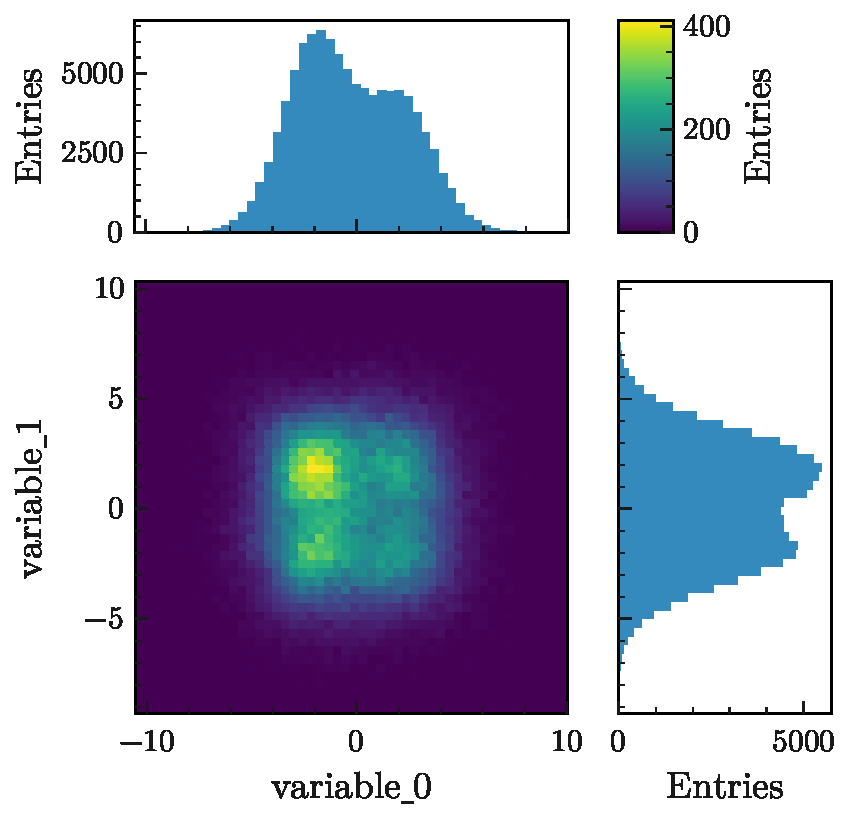
\includegraphics[width=0.75\textwidth]{figs/2d_hist_with_projections.pdf}
\caption{This is a caption.}
\label{fig:probability}
\end{figure}

\begin{table}[bt]
\caption{This is a caption.}
\begin{center}
\begin{tabular}{lll}
Name & Definition & Alternative names \\
\midrule
Purity & \textfrac{TP}{Predicted Positive}=\textfrac{TP}{TP+FP} & Precision \\
Efficiency & \textfrac{TP}{Real Positive}=\textfrac{TP}{TP+FN} & Recall, True Positive Rate \\
False Positive Rate & \textfrac{FP}{Real Negative}=\textfrac{TP}{FP+TN} & \\
\bottomrule

\end{tabular}
\end{center}
\label{tab:probability}
\end{table}

\chapter{Conclusion} \label{sec:conclusion}
This is a conclusion.


% Bibliography
\newpage
\printnoidxglossary[title=List of acronyms, toctitle=List of aronyms, type=acronym]
\printacronyms
\bibliographystyle{plain}
\bibliography{include/bibliography}

\end{document}
